%% Requires compilation with XeLaTeX or LuaLaTeX
\documentclass[10pt,xcolor={table,dvipsnames},t]{beamer}
\usetheme{UCBerkeley}

\title[Your Short Title]{Lab Report (Week 1)}
\subtitle{Proving a phase transition in cellular automata under
asynchronous dynamics}
\author{Alireza Abrehforoush}
\institute{Isfahan University of Technology}
\date{Wednesday, April 20, 2022}

\begin{document}

\begin{frame}
  \titlepage
\end{frame}

% Uncomment these lines for an automatically generated outline.
%\begin{frame}{Outline}
%  \tableofcontents
%\end{frame}

\section{Introduction}

\begin{frame}{Introduction}

\begin{itemize}
  \item Your introduction goes here!
  \item Use \texttt{itemize} to organize your main points.
\end{itemize}

\begin{block}{Examples}
Some examples of commonly used commands and features are included, to help you get started.
\end{block}

\end{frame}

\section{Some \LaTeX{} Examples}

\subsection{Mathematics}

\begin{frame}{Readable Mathematics 42}

Let $X_1, X_2, \ldots, X_n$ be a sequence of independent and identically distributed random variables with $\text{E}[X_i] = \mu$ and $\text{Var}[X_i] = \sigma^2 < \infty$, and let
$$S_n = \frac{X_1 + X_2 + \cdots + X_n}{n}
      = \frac{1}{n}\sum_{i}^{n} X_i$$
denote their mean. Then as $n$ approaches infinity, the random variables $\sqrt{n}(S_n - \mu)$ converge in distribution to a normal $\mathcal{N}(0, \sigma^2)$.

\end{frame}


\subsection{Tables and Figures}

\smallframetitle

\begin{frame}{Tables and Figures}

\begin{itemize}
\item Use \texttt{tabular} for basic tables --- see Table~\ref{tab:widgets}, for example.
\item You can upload a figure (JPEG, PNG or PDF) using the files menu. 
\item To include it in your document, use the \texttt{includegraphics} command (see the comment below in the source code).
\end{itemize}

\begin{table}
\centering
\begin{tabular}{l r}
\tableheadrow
\tableheadcol{Item} & \tableheadcol{Quantity} \\
Widgets & 42 \\
Gadgets & 13
\end{tabular}
\caption{\label{tab:widgets}An example table.}
\end{table}

\end{frame}

\begin{frame}
\frametitle{Figure Example}

Commands to include a figure:

\begin{figure}
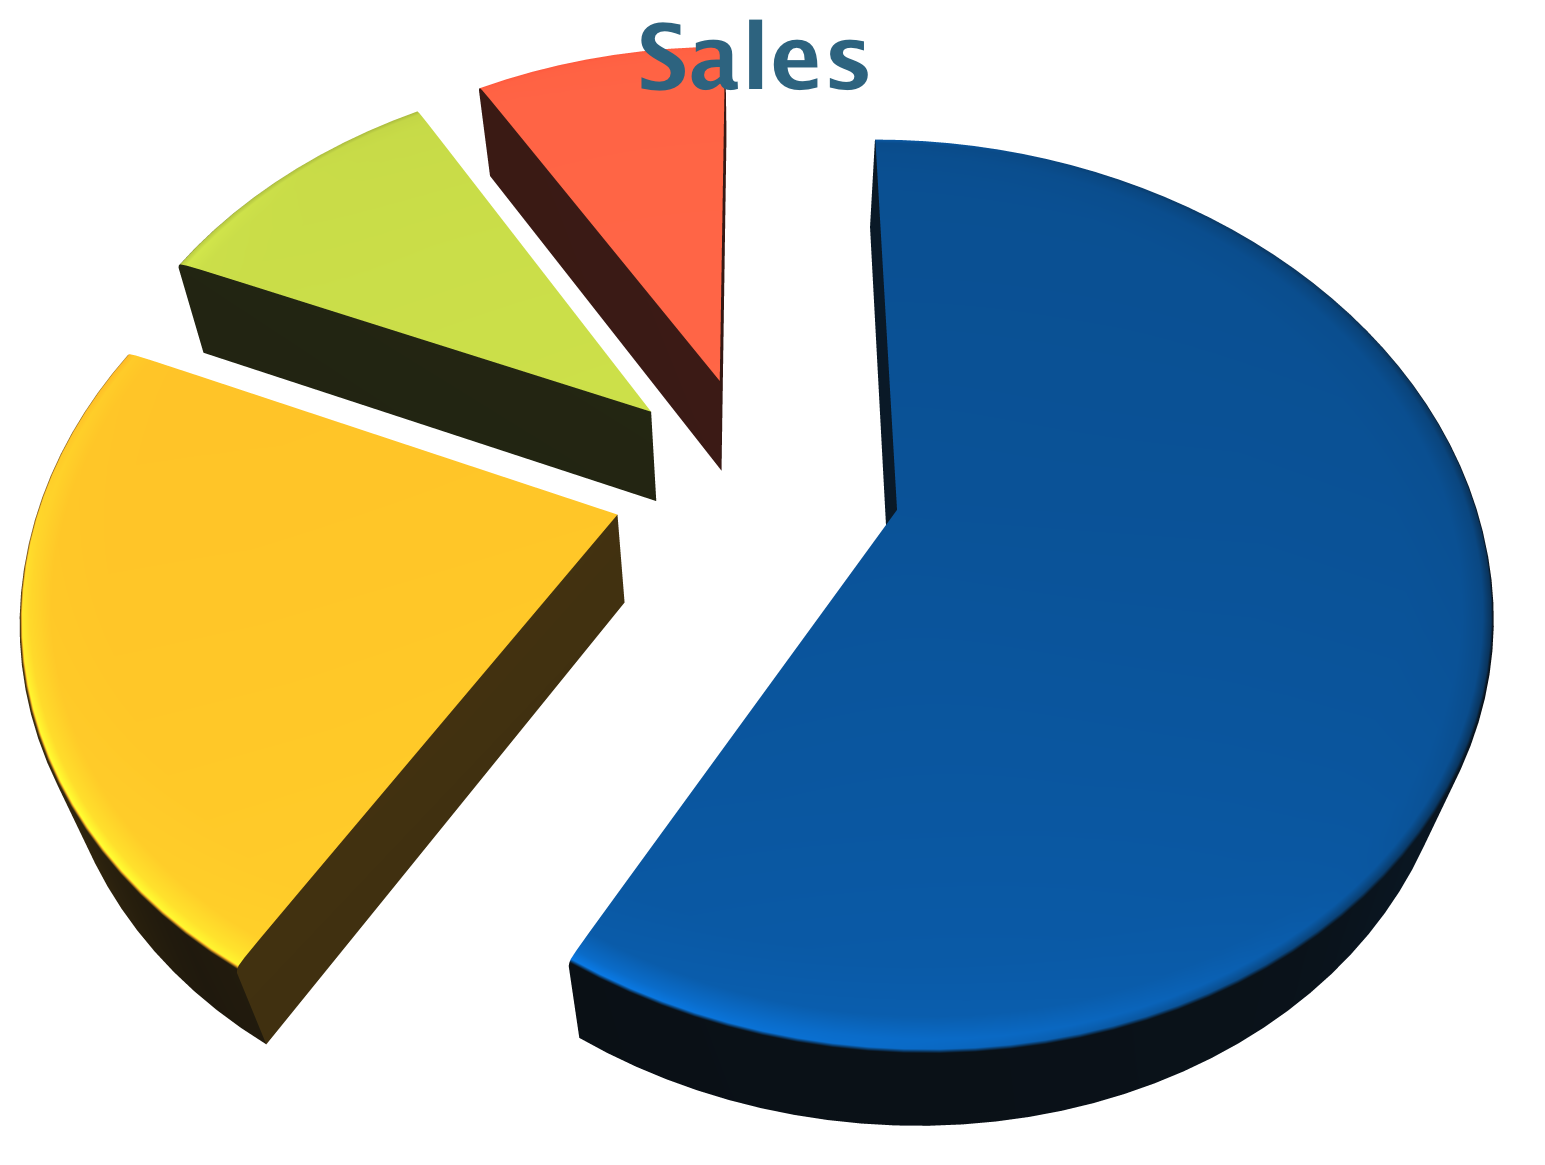
\includegraphics[width=0.4\textwidth]{chart}
\caption{\label{fig:your-figure}Caption goes here.}
\end{figure}
\end{frame}

\begin{frame}
\frametitle{Text in Two Columns}

\begin{columns}[T]

\begin{column}{0.48\textwidth}
\small
Lorem ipsum dolor sit amet, consectetur adipiscing elit. Fusce sit amet massa in dolor pellentesque tempor. Integer nunc. 
\end{column}

\begin{column}{0.48\textwidth}
\begin{itemize}
\item First bullet goes here
  \begin{itemize}
  \item Secondary bullet goes here
    \begin{itemize}
    \item Tertiary bullet goes here
    \end{itemize}
  \end{itemize}
\end{itemize}
\end{column}

\end{columns}
\end{frame}

\normalframetitle

\begin{frame}
\frametitle{Lorem Ipsum}


\includegraphics[width=.65\textwidth,height=.5\textheight]{photo}

\end{frame}


\end{document}
